\documentclass{article}
\usepackage{amsmath,amsthm,graphicx,hyperref}
\newtheorem{theorem}{Theorem}
\begin{document}
\section{Start}\label{sec:start}
Forward to \autoref{fig:plot}, Table~\ref{tab:data}, \eqref{eq:energy}, Theorem~\ref{thm:main}
and Section~\ref{sec:end}. \textbf{Bold link to \ref{sec:end}} and again \ref{sec:end}.
Undefined: \ref{sec:nowhere} and \eqref{eq:nowhere}.
\begin{itemize}
\item In a list: \ref{tab:data} and \href{https://example.org/list}{a list link}.
\end{itemize}
\section{Middle}\label{sec:a}
\subsection{Same name}\label{sec_a}
\subsection{Digits}\label{1abc}
\subsection{Long}\label{sec:a-very-long-label-name-that-goes-beyond-forty-characters}
\subsection{Again}\label{sec:a-very-long-label-name-that-goes-beyond-forty-characters-too}
\begin{figure}[h]
\centering
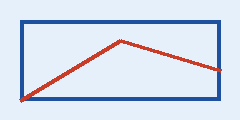
\includegraphics[width=2cm]{plot.png}
\caption{A plot}\label{fig:plot}
\end{figure}
\begin{table}[h]
\centering
\caption{Data}\label{tab:data}
\begin{tabular}{ll}
a & b \\
\end{tabular}
\end{table}
\begin{equation}
E = mc^2 \label{eq:energy}
\end{equation}
\begin{theorem}[Main]\label{thm:main}
Every link resolves.
\end{theorem}
Links: \url{https://example.com/a?b=1&c=2}, \href{mailto:info@example.com}{mail},
\href{javascript:alert(1)}{script}, \href{file:///etc/passwd}{file} and \href{notes.pdf}{relative}.
Internal: \hyperref[sec:start]{back to the start}.
\section{End}\label{sec:end}
Backward to Section~\ref{sec:start}, \ref{sec:a}, \ref{sec_a}, \ref{1abc},
\ref{sec:a-very-long-label-name-that-goes-beyond-forty-characters},
\ref{sec:a-very-long-label-name-that-goes-beyond-forty-characters-too} and \autoref{eq:energy}.
\label{sec:end}
\end{document}
